\documentclass[main.tex]{subfiles}

\begin{document}
\chapter{Literature Review}
\chaplabel{literatureReview}
\textcolor{red}{Need a paragraph to introduce the lit review chapter, why we are doing a lit review and what it will cover}

\section{Signal Processing}
\seclabel{splitreview}
%Implementation of autonomous detection and classification of subsurface objects, with a focus on identifying objects with a high likelihood of being a landmine. interpretation of the output signals from the GPR and metal detector will be processed with the aim to identify and confirm with a percentage the likelihood of a threat. Supplied data sets will be used to create and tune a detection algorithm to meet this goal, and operational trials will be conducted to test the effectiveness of the developed system.
% 
\subsection{Ground Penetrating Radar for mine detection}
\seclabel{gpr}
\subsubsection{Hardware configuration influence on detection capability}
\textcolor{green}{signal noise is introduced at all locations where a change in density occurs. This is considered noise for the purposes of the GPR application - as the signal response does not correlate to the object being searched for; but is not noise in the general sense as the signal does correlate to another density change.}

Radar frequencies are attenuated by underground objects as they absorb the energy in the transmitting signal, dampening the possible response to the receiving antenna. This is particularly problematic in particular soil types, notably wet soils and clays that have a significant damping effect on the radar pulses. Increasing the power of the transmitted signal or increasing the gain on the receiving signal both serve to reduce the effects of ground attenuation and allow for greater scanning depth with GPR. The ability to increase both of these factors is limited by the capacities of the controlling electronics, which in turn is limited by the state-of-the-art of amplifier technologies. This places an effective limit on the scanning depth allowable with GPR technology. \textcolor{green}{what is it?}. Increasing the receiver gain also has the affect of amplifying any noise generated through the system, making the ability to detect subsurface objects heavily constrained by the ability to process and interpret the received signals to differentiate objects of interest from \textcolor{green}{chaff}. Due to the attenuation of the radar signal through the soil, and the limits on the receiving signal gain - a trade-off exists between the maximum sensing depth and the detection resolution.

Wideband frequency coverage is a radar scanning strategy which can be used to achieve high resolution scanning and high depth capabilities, overcoming the limitations of the control electronics. As different frequencies experience different levels of attenuation, a lower frequency transmitter and receiver (~200 MHz) will be capable of detecting at greater depths than a high frequency, at the sacrifice of detection resolution. Conversely high frequency systems (~3 GHz) will achieve greater resolution at the cost of severe attenuation with increased depth. Wideband frequency coverage is the application of antennas which are capable of varying their frequency to allow a single device to scan over a wide frequency band. By collating detection results from multiple frequencies a combined response can be created, which has signal responses from large, deep objects while retaining the ability to distinguish small objects at shallow depths. 

A limitation restricting the application of GPR technology for the purposes of UXO scanning is the small search area. The detection of subsurface objects is effectively limited to objects situated between the transmitting and receiving antennas, which in practice must be only a small distance apart due to signal attenuation. This prevents the scanning of wide fields by placing the antennas a wide distance apart. Iterative scanning must be employed to cover a zone, and with a small scan width this requires a great number of scans.

\textcolor{green}{After re-reading i get what you meant rac about this being close to benchmarking. I've removed any mention of this being an actual commercial device and focused on the important parts to make it more literature review appropriate. --}
The limitation of a single radar scanline has been overcome with the use of an array of transmitting and receiving antennas combined into a single scanning device. Under this arrangement the series of transmitting and receiving antennas are displaced laterally from each other along the length of the device, as shown in \figref{arraylayout}. The application of multiple transmitting and receiving pairs allows for a single pass to scan a significant width, limited only by the number of transmitting and receiving pairs \parencite{3dradarDX}. The proximity of the transmitting pairs also allows for the signal difference at the receiving antennas to be interpreted from multiple transmitters - greatly increasing the fidelity of the scan. The effective sensing locations by pairing each receive antenna to two transmitting antennas are shown as red dots in \figref{arraylayout}.
\begin{figure}[ht]
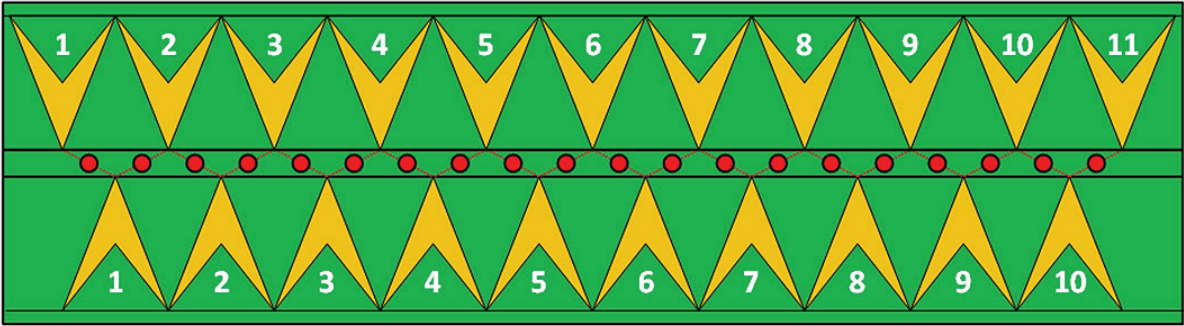
\includegraphics[width=0.8\textwidth]{3-LiteratureReview/3d-radar.png}
\centering
\caption[Example layout of transmitting (bottom row) and receiving elements (top row) of a 3D radar system]{Example layout of transmitting (bottom row) and receiving elements (top row) of a 3D radar system \parencite{3dradarDXG}} \figlabel{arraylayout}
\end{figure}
A scanning device of this kind would be far more costly than a radar system that was only capable of producing a single scanline \textcolor{green}{elaborate?}.

\subsubsection{Signal processing and determination of objects of interest}
\textbf{\textcolor{green}{I think this section is done - and done well. Please tear it apart as mercilessly as possible ASAP, so that I can get an idea of everyone elses expectations/views on how things should be.}}

Typically the processing chain for ground penetrating radars used for landmine detection detection purposes consists of preprocessing (which is extended in comparison with conventional GPR case with a clutter supression stage), initial detection (or primary detection or area selection), where all suspicious anomalies of the subsurface are selected, and discrimination, in which these anomalies are analysed and classified as targets or friendly objects \parencite{Ho.etal2004}. This process requires determining a set of classification characteristics which suitably and uniquely identify the characteristics of an object of interest. These characteristics are limited by those which can be accurately measured by the GPR device, and are commonly the size and shape of the object and other physical aspects. However, objects can also be identified from the raw signal without needing to link parameters to real-world object characteristics, by identifying objects by particular patterns present in the time-frequency plane at the receiving antenna. 

Detection of landmine responses with GPR data is made difficult by the low signal to noise ratio, making preliminary filtering difficult \parencite{Yarovoy2009}. The largest noise component of the received signal is the response due to the air-ground interface, which generates a strong response which can obscure the features of objects of interest which only generate a small signal \parencite{Yarovoy2009}. As a result, minimal elevation of the GPR device is desirable as this minimises the influence of this air-ground interface reflection on the received data. Noise is further reduced from the received signal through statistical tests applied over successive scans, such as Kalman filters, artificial neural networks and fuzzy logic tests \textcolor{green}{cite cite cite}. These algorithms form the preprocessing stage of the processing chain described above.

The easiest way to detect an object is if the objects approximate response is previously known, such as from a model or training data set \parencite{Yarovoy2009}. Algorithms have been developed which identify pattern matches between a known expected response and the received response from the GPR. The most popular algorithm for this application is the inverse-matched filter, which is a mathematical convolution over the received signal to attempt to detect the presence of the expected response \parencite{Osumi1984}. More advanced algorithms are capable of producing results with greater accuracy when correlated with detection confidences from nearby samples. If a number of samples in a local area show high confidence in a detected object the overall confidence that a detection has occurred increases when compared to an isolated positive detection. The hyperbola detection method attempts to identify the hyperbolic shape formed in a visual image when multiple samples are combined in this manner (as in \figref{GPRsample}), through the use of computer vision techniques such as edge detection and the randomised Hough transform \parencite{Xu1990}.
\begin{figure}[ht]
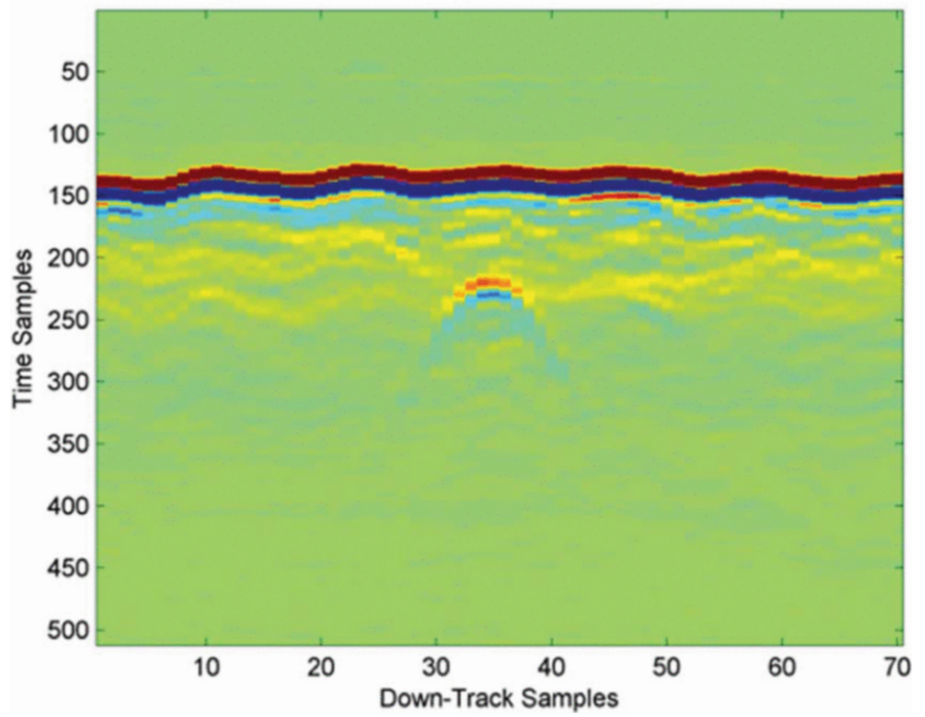
\includegraphics[width=0.7\textwidth]{3-LiteratureReview/GPR-sample.png}
\centering
\caption{Sample GPR response over buried AT mine showing parabolic shape in received signal over object of interest, which can be detected using the randomised Hough transform method} \figlabel{GPRsample}
\end{figure}
These algorithms represent the initial detection stage of the processing chain. Further classification of objects to reduce false-positive testing is possible through artificial intelligence strategies such as neural networks or decision trees, which require extensive sets of training data to produce strongly confident results, or through the pairing of the GPR detection with detection confirmation from a secondary sensor, such as a metal detector.

\subsection{Metal detectors for mine detection}
A metal detector operates on a similar arrangement of equipment as a GPR unit, with both systems utilising a transmitting source and a receiving device to detect objects. Metal detectors that operate on the eddy current principle generate magnetic fields which penetrate the soil, inducing eddy currents in underground metallic objects. These eddy currents in turn generate a secondary magnetic field, at a greatly reduced amplitude, which can then be detected by the receiving coil of the metal detector \parencite{Candy2008}. Similar to the GPR, the signal to noise ratio is low, especially in heavily mineralised soils, and all signals are heavily attenuated with depth \parencite{Candy2008}.

Detection of metal using metal detectors that operate on the eddy current principle is typically performed by an operator. On consumer marketed devices, received signals from the metal detector are converted directly to an audio signal, at which point the operator can distinguish metal objects from non-metals by the amplitude and tone of the received signal. Using this method a qualified deminer can readily locate the position of a subsurface object, however full classification of the object or determination of its parameters such as size, shape and material is practically impossible \parencite{Kruger2006}. Some degree of basic automatic classification is common on devices marketed for treasure hunting, where it is used to distinguish valuable metallic objects from common metals. This classification is known as a discriminated signal and is possible due to the variation in eddy currents induced by different metals - most particularly between ferrous and non-ferrous metals. 

The signal response that allows the creation of the discriminated signal is the time constant of the received audio sample. The time constant is a function of the metallic material being detected, based largely on the target inductance and conductivity \parencite{Candy2008}. Selectively discriminating times when the signal's time constant meets a certain criteria allows for the detection of different metal types, with most ferrous targets having very long time constants, and targets composed of other metals being able to be discriminated based on expected time constant range \parencite{Candy2008}. This method however is not generally applicable to the purposes of mine detection, as the size and shape of a material can influence the time constant, and the method is not reliable in the case of small composite metal parts of different material and complex shape, which mines usually consist of \parencite{Kruger2006}. The influence of mineralised soil is also not compensated for by the discriminator which would also affect the determination of metal type \parencite{Kruger2006}.

A method more appropriate for mine detection, and particularly automatic mine detection, is the generation of signatures of mine objects from a sample of training data sets. A signature of an object can be generated from the phase loop representation of the sample signal in the complex plane, an advantageous strategy as the required signal to noise ratio for a quality signature is low \parencite{Kruger2006}. Example object signatures showing the variance between objects are shown in \figref{signature}.
\begin{figure}[ht]
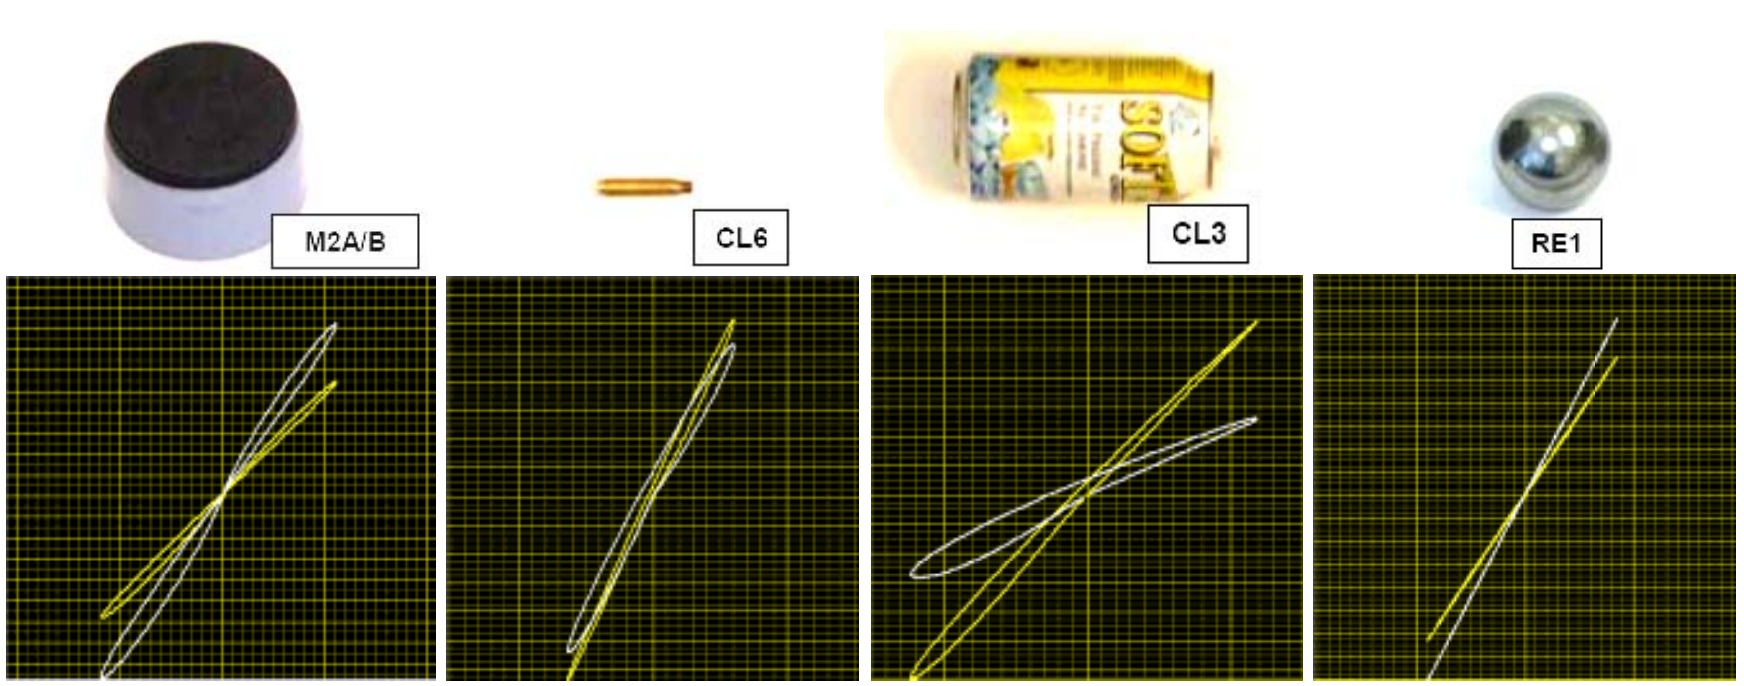
\includegraphics[width=0.8\textwidth]{3-LiteratureReview/signature.png}
\centering
\caption[Phase plot signatures of various potential subsurface objects - a landmine, bullet casing, soft drink can, steel ball (from left to right)]{Phase plot signatures of various potential subsurface objects - a landmine, bullet casing, soft drink can, steel ball (from left to right) \parencite{Kruger2006}} \figlabel{signature}
\end{figure}
This signature is capable of uniquely identifying an object type (to a certain degree) allowing comparison of detected samples against a limited set of known signatures, yielding an object classification. The low signal to noise ratio requirement also means that the strategy is reasonably robust against depth based attenuation, allowing consistent classification of objects irrespective of depth. This result is shown in \figref{comp-signature}. \Figref{comp-signature} also highlights the requirement for ground signal compensation to allow for correct matching of signatures. The ground compensation process is similar to that described for GPR technology. Important to note is that the ground compensation algorithm used on the samples must be identical to the ground compensation algorithm used to generate the signatures from the training set to guarantee comparability \parencite{Kruger2006}.
\begin{figure}[ht]
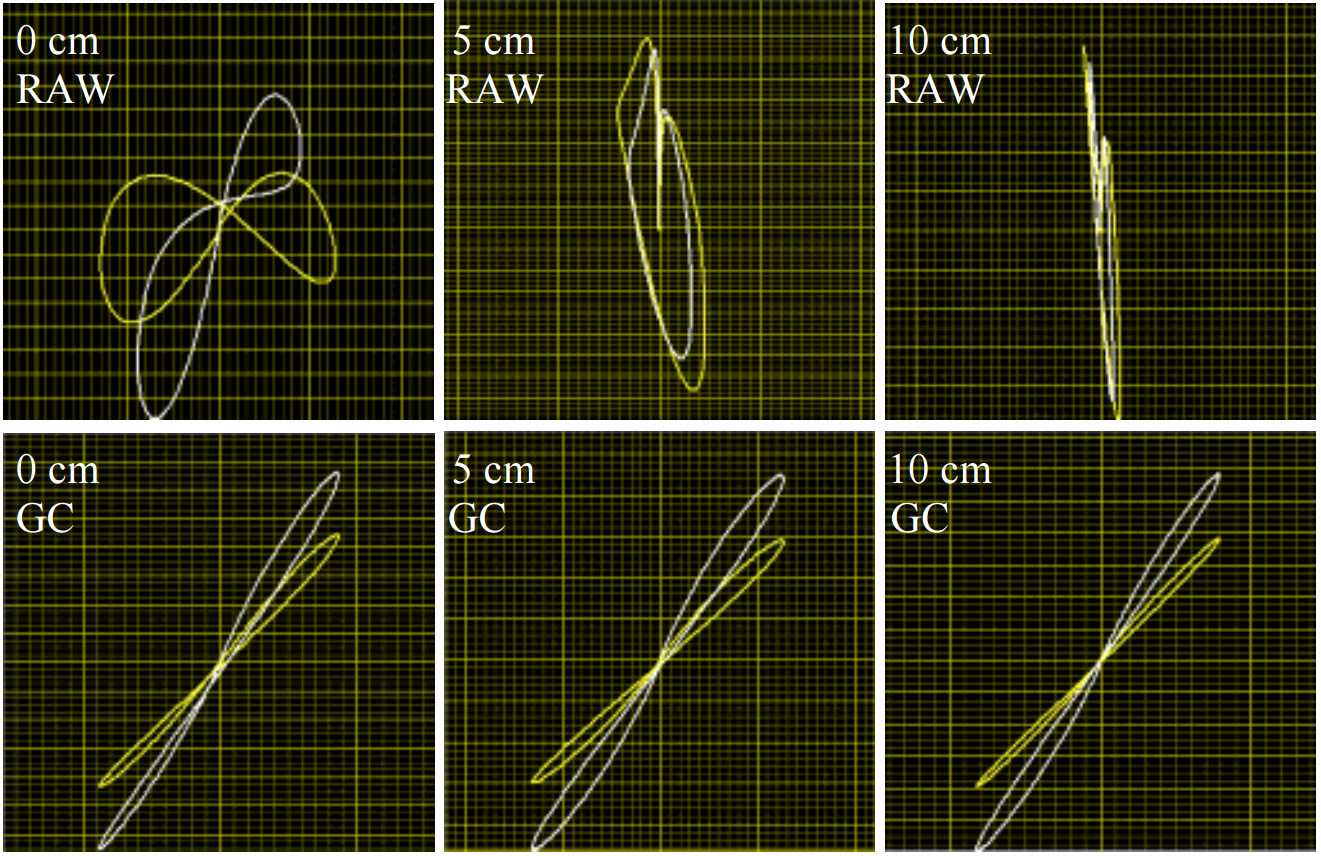
\includegraphics[width=0.8\textwidth]{3-LiteratureReview/compensated-signature.png}
\centering
\caption[Phase plot signatures of a landmine at varying depths. The top row shows the raw data phase plot and the bottom row shows the ground compensated signal]{Phase plot signatures of a landmine at varying depths. The top row shows the raw data phase plot and the bottom row shows the ground compensated signal \parencite{Kruger2006}} \figlabel{comp-signature}
\end{figure}
The signature method has a notable failure point where the presence of a metallic non-mine object situated immediately next to a mine can interfere with the signature of the received sample, reducing the likelihood that a correct identification will be made. This is particularly problematic where large metallic objects can completely obscure the signature of smaller objects. As a result, this technique is limited to situations in which metallic contamination is sparse, or metallic objects are typically an order of magnitude smaller than the objects of interest \parencite{Kruger2006}.

\subsection{Application of multiple sensors in mine detection}
The wide range of potential materials, shapes and burial depths of dangerous underground objects and the constraints of sensing technologies means that single sensor based systems are limited in their detection capacity \parencite{Yarovoy2009}. Combination sensing allows access to a wider gamut of information about a particular subsurface object, allowing detection of a wider range of objects and heightened confidence in the detection rate of mines and IEDs. Two potential configurations exist - where a single sensor is used as a primary detector with confirmation provided by secondary sensor, and where both sensors are used concurrently and information from both detectors is processed simultaneously. Mutual processing of the data from both sensors is called sensor fusion. A common distinction is made between potential levels of sensor fusion \parencite{Yarovoy2009}:
\begin{itemize}
\item \textbf{Decision-level fusion:} information from the sensors is evaluated individually and a decision is made (mine or non-mine) for each sensor. Confidence in the sensor's independent decision is compared against the decision vector to produce a final determination.
\item \textbf{Feature-level fusion:} information from the sensors is produced from the raw sensor data individually. This information is then combined from all sensors to create a singular feature, with a single and final determination made against this feature. 
\item \textbf{Data-level fusion:} data is combined from all sensors to produce a single set of information about the feature. A final determination is made against this feature.
\end{itemize}
Features are linked between sensors by associating samples across multiple sensors, generally by proximity. Features detected by different sensors within a certain threshold distance of each other are associated and considered as the same feature. Each progressive step down from decision-level fusion requires significantly greater computational processing, and greater knowledge of the sensor dynamics and the correlations of signal features to real-world object parameters \parencite{Yarovoy2009}. Higher level fusion strategies lend themselves well to machine learning techniques, which can be naive to the sensor mechanics and produce correlations based on learned sample data sets computationally cheaply. Experimental trials suggest that all forms of sensor fusion are capable of producing significantly more accurate detection results with far fewer false-positive incidents than single sensor systems \parencite{Yarovoy2009}.

\section{Navigation and Automation}
\seclabel{navigationandautomation}
\subsection{Autonomous control of the quad bike}
\textcolor{green}{I wanted to chuck something in here about PID control cos thats what we're gonna be using to control the vehicle from the waypoints. We may not end up having word count spare but if we do i think a bit of background here won't go astray.}

\subsection{Path Tracking}
\seclabel{pathTrackingLitReview}
Path tracking uses location information from a GPS or some other positioning system to guide a vehicle along a pre-defined course. In theory the path can be defined as a continuous function but this is inefficient in practice. Instead, a path is discretised and defined by a series of points, called waypoints (shown in \figref{pathDefining}). A path can either be described as lines connecting the waypoints or as a series of closely spaced waypoints. Due to the implementation of path tracking systems on digital devices the path description will be discretised at some point and so the definition has no impact on the application of the methods described below \parencite{Giesbrecht2005}.
\begin{figure}[ht]
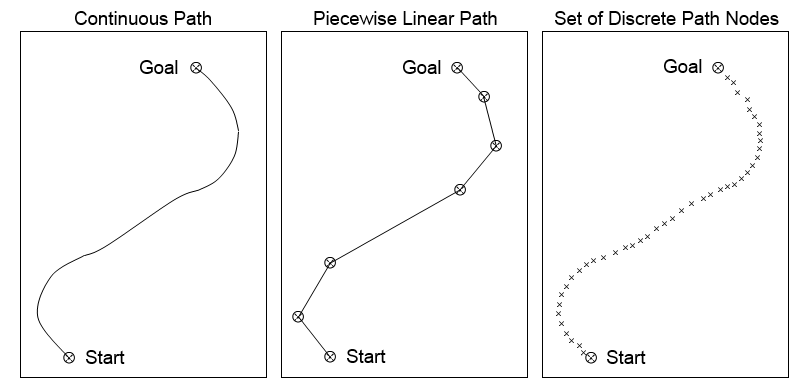
\includegraphics[width=0.9\textwidth]{3-LiteratureReview/pathDefining.png}
\centering
\caption[Various ways to define a path]{Various ways to define a path \parencite{Giesbrecht2005}} \figlabel{pathDefining}
\end{figure}

\subsubsection{Geometric Path Tracking}
Geometric path tracking uses geometric relationships between a vehicle and a path to produce a control algorithm as a solution to the problem. Theories assume vehicles use the Ackermann method for steering so a simplified steering model can be used for the geometry. This reveals a relationship between the steering angle and the curvature that the non steering wheels will follow. Two of the most commonly used geometric vehicle models are Pure Pursuit and the Stanley Method \parencite{snider2009}.

Pure Pursuit uses a path 'look-ahead' distance to measure the future error between the vehicle and the path in real time which can then be steered to and corrected for. \Figref{purePursuitGeom} shows the geometry associated with Pure Pursuit at one point in time. It shows a goal point $(g_x, g_y)$ on the desired path at a specified look-ahead distance $l_d$ in front of the vehicle. The steer angle is calculated based on an arc that would connect the centre of the non-steering axle to the goal point. The calculation of the goal point is effectively adding a waypoint to the path at that point. When high curvatures are present in a path the controller may begin to cut corners due to a look-ahead distance that would effectively skip this portion of the path. Lateral error on a path of constant curvature may also be experienced due to geometric controller characteristics which do not take into account the curvature of a path. However, Pure Pursuit provides a very robust tracking algorithm when discontinuous curvatures are present \parencite{snider2009}. In general, for more accurate tracking a short look-ahead distance should be used but will eventually result in oscillation, for smoother tracking a long look-ahead distance should be used but this will reduce precision \parencite{snider2009}.
\begin{figure}[ht]
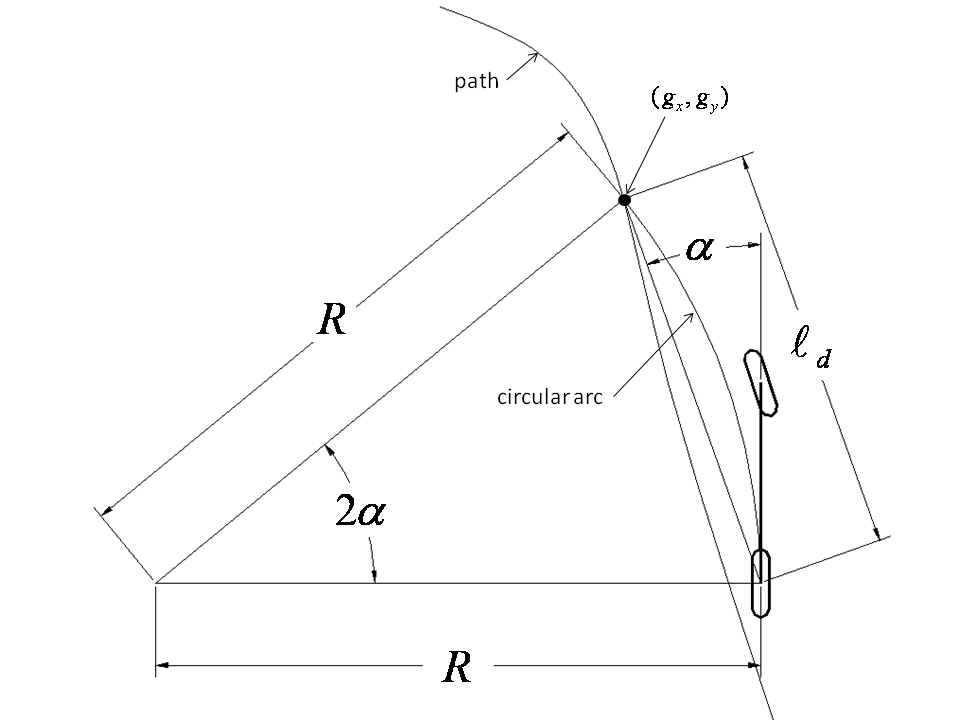
\includegraphics[width=0.6\textwidth]{3-LiteratureReview/purePursuitGoal.png}
\centering
\caption[Pure Pursuit Geometry]{Pure Pursuit Geometry \parencite{snider2009}} \figlabel{purePursuitGeom}
\end{figure}

The Stanley Model uses the lateral error between the centre of a wheels axle and the nearest path point  to determine steer angle (\figref{stanleyGeom}). It is simply set to the heading error which is given as the difference between the vehicles heading and the instantaneous heading of the nearest point on the path, $\theta_e$. An extra term is used when the lateral error is non zero which amplifies the steer angle to a new value of $\delta$.  This gives an effect so that as the error increases, or as the vehicle strays further from the path, the wheels steering angle is amplified in an attempt to correct for this error. The Stanley Method is very well suited to higher speed tracking but can run into problems when curvature discontinuities are present in the path.
\begin{figure}[ht]
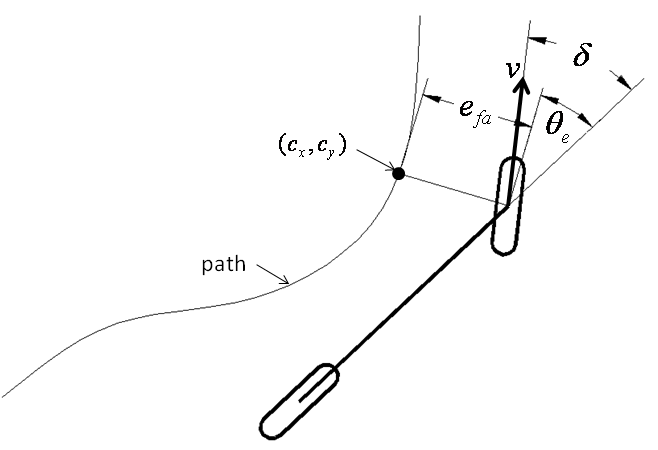
\includegraphics[width=0.5\textwidth]{3-LiteratureReview/stanleyMethod.png}
\centering
\caption[Stanley Method Geometry]{Stanley Method Geometry \parencite{snider2009}} \figlabel{stanleyGeom}
\end{figure}

Some limitations of geometric path tracking methods are related to the dynamics of a vehicle which are not present in the theory, namely the capabilities of a platform and its actuators. Due to this the method expects an instant response from elements such as the steering which is an issue when high path curvatures are present or when the curvature of the path suddenly changes. As a result the method cannot guarantee that the vehicle will follow a path as accurately as designed and at high speeds that vehicle may skid or tip \parencite{coulter1992}.

\subsubsection{Kinematic Path Tracking}
The kinematic model collapses a four wheeled vehicle into a two wheeled model, much like the geometric path tracking approach. The equations of motion for the simplified system are then used to relate the vehicle speed, change in heading error and change in lateral error to a user defined velocity and steer angle in path coordinates. In practice, the same trade off between performance and stability is apparent as in the geometric models, accurate tracking at low speeds but problems due to neglected dynamics at high speeds \parencite{snider2009}. This method is not as robust as Pure Pursuit and displays a similar behaviour to the Stanley Method when discontinuities in curvature are present.

\subsubsection{Dynamic Path Tracking}
A dynamic model approximates the real dynamics of a vehicle which was one of the downfalls of the previous examples. Similar to the kinematic model, the vehicle speed, heading error and lateral error are related to a user defined velocity and steer angle in path coordinates. Even though the dynamics of the vehicle are included in this model, extreme path dynamics such as large changes in curvature can have as much of an effect on the efficiency of the path tracking as before\parencite{snider2009}. Discontinuities in the path still have a noticeable effect on accuracy and the steady state lateral error is still present. However, in a more realistic scenario a dynamic path tracking method does show overall improvement \parencite{snider2009}.

\subsection{Turning the Platform a Specified Angle}
In a path similar to that described by the piecewise linear definition, a turn can be moderately controlled by introducing a variable called the radial tolerance \parencite{Giesbrecht2005}. The radial tolerance describes the distance from the waypoint at which the system considers that waypoint 'reached', ultimately changing the point at which the platform will begin the turn towards the proceeding waypoint. If the radial tolerance is set too large the platform will begin the turn early resulting in poor path tracking. If the radial tolerance is set too small the platform will overshoot the desired path due to unaccounted vehicle dynamics and/or restrictions in steering angle. \Figref{waypointTolerances} shows examples of a radial tolerance set slightly too low (1 metre) in blue and more realistically in grey (6 metres) for a vehicle following the path in red with a turn radius of 4 metres. It is easily visible that both methods are unable to follow the desired path with perfect precision due to real vehicle dynamics.

\begin{figure}[ht]
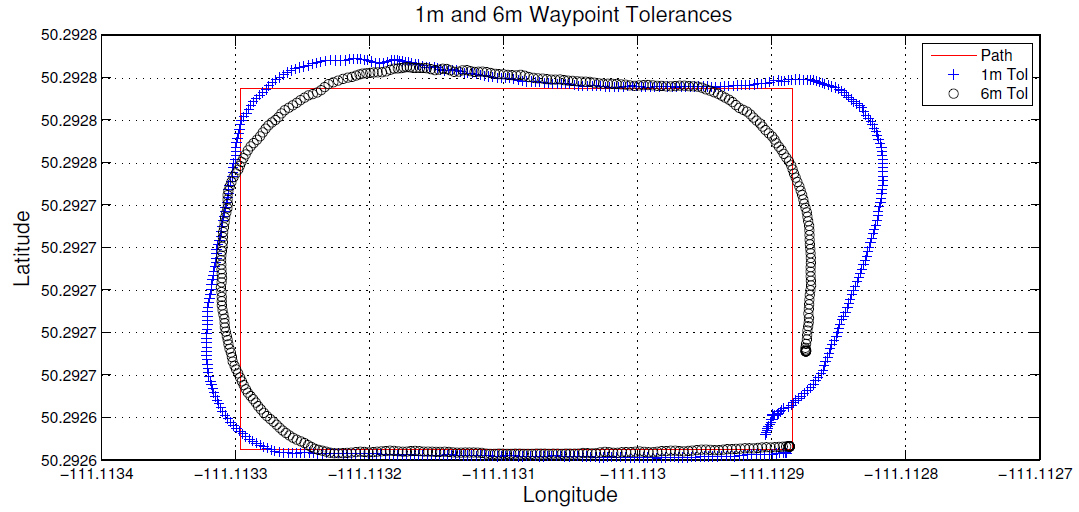
\includegraphics[width=\textwidth]{3-LiteratureReview/waypointTolerances.PNG}
\centering
\caption[Effect of Waypoint Tolerances on Path Tracking]{Effect of Waypoint Tolerances on Path Tracking \parencite{Giesbrecht2005}} \figlabel{waypointTolerances}
\end{figure}
























\end{document}